\begin{frame}{Protein-promoter interactions}
% Data for proteins binding to promoters are gathered from Beyer and Workman et al.~\cite{BeyerWorkman2006}. It is a table of 13,239 transcription factor to gene interactions from 158 transcription factors, where each interaction has an assigned p-value.
Beyer and Workman et al.~\cite{BeyerWorkman2006}: 138 TFs (10,484 edges) \\
Yeastract~\cite{yeastract2017}: 173 TFs (136,813 edges)
\begin{figure}[ht]
  \centering
  \begin{subfigure}[t]{0.38\textwidth}
  \centering
  \caption{}
  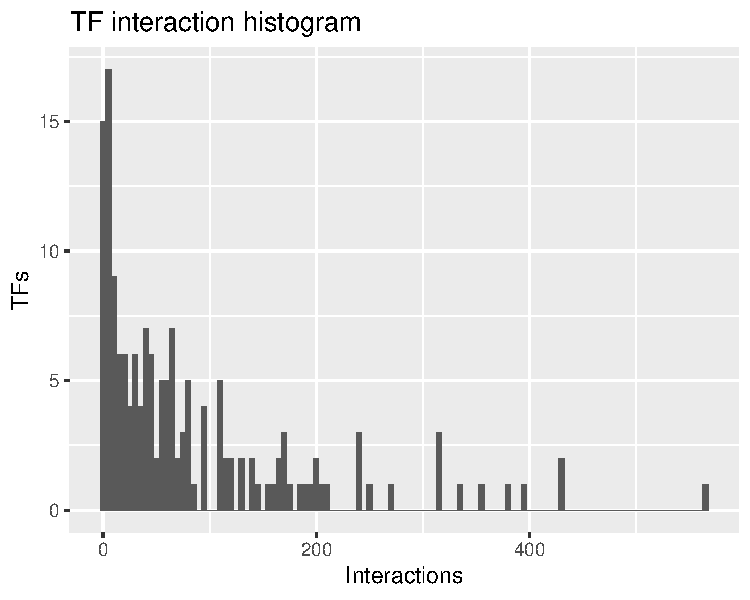
\includegraphics[width=\textwidth]{data/fig/TF_interaction_hist.pdf}
  \label{fig:TF_interactions_hist}
  \end{subfigure}
  \hfill
  \begin{subfigure}[t]{0.5\textwidth}
  \centering
  \caption{}
  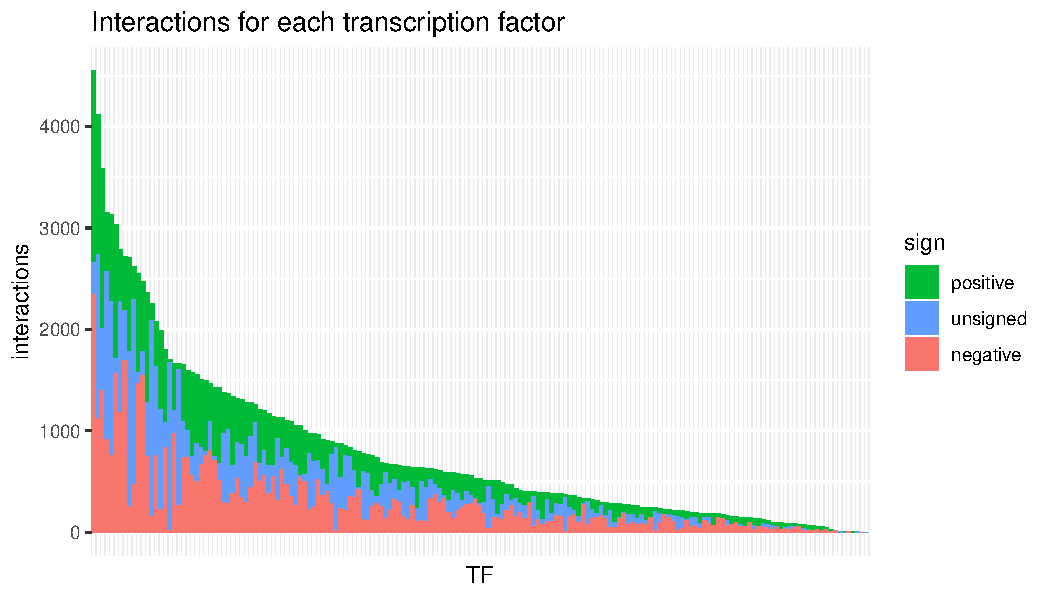
\includegraphics[width=\textwidth]{data/fig/yeastract.pdf}
  \label{fig:yeastract}
  \end{subfigure}
  \caption{\textbf{TF interactions.} TF$\rightarrow$gene interaction histogram for Beyer-Workman (a), and individual TF interactions for Yeastract (b). }
\end{figure}
% Most TFs in the data has in the range of ${\sim}10$ genes they are known to regulate but some regulate in the range of hundreds~(\autoref{fig:TF_interactions_hist}).
% The processed RNA values in \autoref{sec:yeast_data} have 5881 measurements for 266 TF knockout experiments, so not all knocked out TFs have known edges from this protein-promotor dataset. The overlap between the datasets reduces the number of edges from 13,239 to 10,484 with 128 of the 266 TFs having no known regulon. 
% The counts of different types of interactions for each of the 173 TFs are summarized in~\autoref{fig:yeastract}. Most TFs has more than 1 interaction and there is generally both activating and repressing interactions for any given TF. The TF with the most interactions is TF with ORF name YLR131C, which regulates 4550 unique genes in this dataset. 
\end{frame}

% \begin{frame}{Protein-promoter interactions - Yeastract}
% % Another dataset for transcription factors binding to DNA was found from Yeastract~\cite{yeastract2017}. The data was found by using the Yeastract website's function "Generate Regulation Matrix" retrieving all TF interactions documented with either DNA binding or expression evidence. The retrieval was performed separately for TFs acting as activator or inhibitor. The search was performed based on the systematic names of TFs and target genes from the TF dataset described in~\autoref{sec:yeast_data}, which is 266 TFs versus 5881 genes. The resulting tap-separated tables listing all regulatory interactions were used after having all the names converted to systematic names, since they are retrieved as popular names. The conversion was performed using Yeastract's own "ORF List to/from Gene List" conversion utility to ensure that all gene identifiers would be converted sucessfully back to ORF naming.
% % It is assumed that it is not known whether the protein-promotor interaction is positive or negative for TF-gene interactions that were listed in both the activator and repressor sets. They become defined here as unsigned edges, while the remaining activator and repressor interactions become defined as positive and negative edges. The counts of unique transcription factors found and TF-gene interactions are summarized in~\autoref{tab:yeastract}.
% \begin{table}[ht]
% \caption{\textbf{Yeastract TF interactions.} processed = assigning overlap in activators and inhibitors to a third "unsigned" category.}
% \begin{tabularx}{\textwidth}{@{}lYYYcYYYY@{}}
%     \toprule
%      & \multicolumn{3}{c}{raw} & \phantom{aa} & \multicolumn{4}{c}{processed} \\
%     \cmidrule{2-4} \cmidrule{6-9}
%      & activator & inhibitor & all && positive & negative & unsigned & all \\
%     \midrule
%     TFs & 170 & 173 & 173 && 167 & 171 & 157 & 173 \\
%     interactions & 85,098 & 94,286 & 179,384 && 42,527 & 51,715 & 42,571 & 136,813 \\
%     \bottomrule
% \end{tabularx}
% \label{tab:yeastract}
% \end{table}
% % The interactions were from 170 unique TFs in both the activator and repressor lists, as well as 3 additional unique TFs in the repressor list. After assigning the interactions a positive, negative, or unsigned edge, the counts of unique proteins remained about the same, indicating that a transcription factor will usually both have activating and repressing roles. There are $173 \cdot 5881 - 173 = 1,017,240$ possible edges from the TFs described in the Yeastract data to all of the measured genes, excluding self-interactions. About 13\% of possible edges are known~($136,813 / 1,017,240 \approx 0.134$), of which about 69\% have a known sign~($(42,527 + 51,715) / 136,813 \approx 0.689$).
% \end{frame}

